\documentclass{article}

\usepackage{listings}
\usepackage{hyphenat}
\usepackage{float}
\usepackage[T1]{fontenc}
\usepackage{hyperref,adjustbox}
\usepackage{graphicx}
\usepackage{pdfpages}
\usepackage[brazilian]{babel}
\usepackage{adjustbox}
\usepackage{multirow}
\usepackage{amssymb}
\usepackage{tabulary}
\usepackage{pifont}% http://ctan.org/pkg/pifont
\newcommand{\cmark}{\ding{51}}%
\newcommand{\xmark}{\ding{55}}%
\usepackage{tikz}
\usepackage{natbib}
\usepackage[T1]{fontenc}
\usepackage{bm}
\usepackage{enumitem}
\usepackage{algorithm}
%\usepackage{arevmath}     % For math symbols
\usepackage[noend]{algpseudocode}
\usepackage{mathtools}

\usepackage{titlesec}
\DeclarePairedDelimiter\ceil{\lceil}{\rceil}
\DeclarePairedDelimiter\floor{\lfloor}{\rfloor}

\titleformat{\section}
{\normalfont\Large\bfseries}{\thesection}{1em}{}[{\titlerule[0.8pt]}]


\title{Trabalho Prático - Identificação de números primos \\
	\large Computação Paralela}

\author{Heitor L. Werneck}
\begin{document}
\maketitle

\section{Introdução}

Um número primo é um número natural maior que 1 que não é produto de dois
números naturais menores. Números naturais maiores que 1 que não são primos são
chamados de número composto. A identificação de um número primo também tem
relação com a função divisora do mesmo, já que os números primos tem exatamente
2 divisores exatos, então com o número de divisores exatos de um número é
possível identificar a primalidade de um número (tarefa um pouco mais complexa
que o teste de primalidade). Em matemática, e especificamente na teoria dos
números, uma função divisora é uma função aritmética relacionada aos divisores
de um inteiro. Quando referida como função divisora, ela conta o número de
divisores de um inteiro (incluindo 1 e o próprio número). Diversas propriedades
matemáticas podem ser observadas atráves da observação da função divisora ao
longo de diferentes amostragens, que pode potencialmente auxiliar matemáticos
nas suas áreas de pesquisas, e talvez até mesmo no caso de um algoritmo
suficientemente eficiente pode ajudar a eliminar ou "reforçar" ainda mais
colorarios existentes na área.

Nesse trabalho será feito a implementação paralela mestre-escravo usando MPI de um algoritmo que identifica números primos em um vetor de N inteiros. Primeiro será mostrado mais detalhes sobre o problema. Além disso será mostrado as soluções como uma visão geral e após isso será apresentado uma documentação do código, as argumentações sobre as decisões das soluções, resultados e análises serão descritos na pénultima seção.

\subsection{Especificação do Problema}
O programa deverá ler o arquivo de entrada deverá e carregado para memoria no
processo mestre. Após o processamento, cada processo escravo deverá retornar
para
o processo mestre quantos divisores exatos possui cada valor armazenado na
sua fatia do vetor. depois que o último escravo terminar, o processo mestre
deverá colocar o número de divisores de cada elemento do arquivo de entrada
em um arquivo de saída (saída.txt) na ordem em que os valores originais
estavam no arquivo de entrada. A tomada de tempo das execuções será
feita somente no processo mestre após leitura do arquivo de entrada e antes
da escrita do arquivo de saída, ou seja,
não será considerado o tempo de
entrada/saída.

A paralelização da aplicação será dividida em 4 partes, as quais terão um relatório técnico. São elas:
\begin{enumerate}
	\item perfil de desempenho sequencial (usando prof)
	\item identificação das oportunidades de paralelização
	\item paralelização
	\item avaliação dos ganhos da paralelização
\end{enumerate}

\subsection{Problema}

Como mostrado na subseção anterior o
problema é simples e consiste em determinar o número de divisores exatos dos elementos $a_i$ de um vetor $A$ de tamanho $N$.

\section{Solução}

Para solucionar esse problema procura-se inicialmente uma função/algoritmo $d(a_i)$ que consiga determinar o número de divisores de um elemento $a_i$.

Esse problema pode ser solucionado facilmente eficientemente com um algoritmo de fatoração de primos atráves da utilização da relação mostrada na Equação \ref{eq:divisorfunction}, que atráves da quantidade de vezes $e_i$ que um número primo aparece em uma fatoração de primos o número de divisores pode ser calculado. Isso é bem simples de entender, já que a fatoração de primos de um divisor $d'$ de $a$ tem que ser um subconjunto da fatoração de primos de $a$, então para o calculo do número de divisores basta calcular todos diferentes subconjuntos da fatoração de primos de um número $a$, o número de diferentes subconjuntos então são calculados usando a Equação \ref{eq:divisorfunction}.

\begin{equation}\label{eq:divisorfunction}
	d(a)=\prod_{i=1}^{k} (e_i+1)
\end{equation}

Agora para a fatoração de primos existem diversos métodos extremamente rebuscados, aqui será utilizado uma abordagem simples, porém de maneira otimizada. Para a fatoração e contagem de divisores será aplicado o algoritmo \ref{alg:divisorfunc} no qual uma lista de primos é percorrida (linha \ref{alg:divisorfunc:for}) e divisões são feitas caso o número seja um divisor e o contador de divisores e atualizado logo após as divisões (linha \ref{alg:divisorfunc:changes}). Para otimizar o método um limite de busca é estabelecido na linha \ref{alg:divisorfunc:end}, já que no caso de a condição ser atendida o número atual é um primo ou é o número 1, denotando que a fatoração pode ser finalizada. Note que nesta proposta não é guardado os fatores, já que não é isso que buscamos, mas sim o número de divisores do número.

\begin{algorithm}
	\caption{Função divisora\label{alg:divisorfunc}}
	\begin{algorithmic}[1]
		\Procedure{d}{$a,primes$}
		\State $num\_divisors\gets 1$
		\For{$i \gets 0$ to $|primes|-1$}\label{alg:divisorfunc:for}
		\State $count \gets 0$
		\If{$number \bm{\bmod} prime = 0$}\label{alg:divisorfunc:changes}
		\While{$number \bm{\bmod} prime = 0$}
		\State $number \gets number/prime$
		\State $count \gets count + 1$
		\EndWhile
		\State $num\_divisors \gets num\_divisors *(count+1)$
		\EndIf
		\If{$prime > \sqrt{number}$}\label{alg:divisorfunc:end}
		\If{$number \neq 1$}
		\State $num\_divisors \gets num\_divisors * 2$
		\EndIf
		\State \textbf{break}
		\EndIf
		\EndFor
		\Return $num\_divisors$
		\EndProcedure
	\end{algorithmic}
\end{algorithm}

Além disso ainda falta o gerador de primos que alimenta o algoritmo \ref{alg:divisorfunc} com uma lista de primos. Para gerar os primos até um limite $n$ foi implementado o crivo de eratóstenes com algumas otimizações para melhorar a performance do algoritmo. O crivo tradicional pode ser visto no algoritmo \ref{alg:erasto}. Na implementação duas otimizações, a primeira delas consiste de começar a marcação a partir do quadrado do primo encontrado e a segunda é a representação somente dos números impares do vetor, assim diminuindo o número de computações em dois e liberando mais memória (aumentando também a chance de cache hit).


\begin{algorithm}
	\caption{Crivo de Eratóstenes\label{alg:erasto}}
	\begin{algorithmic}[1]
		\Procedure{crivo}{$n$}
		\State $A[n+1]$ \Comment{Vetor de tamanho n}
		\State Atribua a todos elementos de $A$ o valor $true$
		\State $A[0]\gets 0; A[1]\gets 0$
		\For{$i \gets 2$ to $\sqrt{n}$}
		\If{$A[i] = true$}
		\State Atribua a todos múltiplos de $i$ até $n$ $false$
		\EndIf
		\EndFor
		\State primes \gets Transforme A em um vetor dos primos encontrados
		\Return primes
		\EndProcedure
	\end{algorithmic}
\end{algorithm}

O diagrama da figura \ref{fig:execoverviewserial} mostra uma visão geral de como cada componente desse se combina para resolver o problema final.

\begin{figure}[htp]
    \centering
    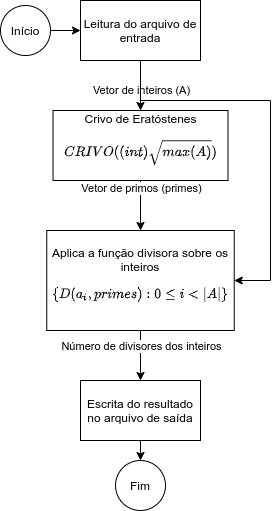
\includegraphics[width=4cm]{./overview_parallel_df}
    \caption{Visão geral da execução.}
    \label{fig:execoverviewserial}
\end{figure}

\section{Solução Paralela}

Com a execução da abordagem demonstrada anteriormente foi possível obter alguns informações sobre oportunidades de paralelização, mais informações sobre os resultados serão detalhados em uma futura seção, por enquanto será focado na solução proposta. A oportunidade mais em vista é a paralelização da aplicação da função divisora, que é uma parte da solução que é embaraçosamente paralela e pode ser aplicado uma abordagem mestre-escravo para melhorar o tempo de execução do algoritmo.

Em questão arquitetural, com o MPI, foi simplesmente feito uma abordagem mestre-escravo, no qual os escravos computam a função divisora em blocos determinados em tempo de execução, que são na prática blocos de tamanhos quase iguais para todos. Com esse método de decomposição de dados, os blocos foram divididos de acordo com as seguintes fórmulas, sendo id o identificador do processo, p o número de processos e n o tamanho total do bloco a ser decomposto.

Primeiro elemento controlado pelo processo id:

\begin{equation}
\floor{\frac{id\cdot n}{p}}
\end{equation}

Último elemento controlado pelo processo id:

\begin{equation}
\floor{\frac{(id+1)\cdot n}{p}}-1
\end{equation}

Para a parelelização no código foi especificamente modificado a linha 18 da função main do arquivo serial.c somente e algumas outras linhas necessárias para o setup do MPI dentro da própria main. A main foi modificada para comportar a configuração do nó mestre (envia e recebe dados) e os nós escravos (envia, recebe e computa). O mestre carrega o arquivo de entrada na memória e envia logo em seguida os blocos do mesmo no qual os escravos alocam dinâmicamente o tamanho e processa-os para gerar os resultados finais.

A proposta de decomposição de dados nessa parte da computação pode trazer muitos ganhos por ser embaraçosamente paralela e também consegue escalar bem pelo mesmo motivo. Espera-se que com uma entrada grande o programa consiga escalar próximo do limite teórico de speed up pela natureza do problema, que leva a menos overhead de comunicação, altamente paralelizável e etc. Mais detalhes sobre o perfil sequencial será explicado em uma seção futura.

\section{Implementação}

Nesa seção será introduzido os módulos com suas respectivas funções, no caso desse problema não foi necessário a construção de nenhuma estrutura de dados. Os tipos primitivos foram suficientes para realizar toda implementação da solução.
\subsection{Utils}

Esse é o módulo que contém as funções útilitarias dos programas, trata entrada e saída de dados assim como algumas transformações de dados.

\begin{enumerate}

    \item int file\_num\_lines(FILE *f)
	
	Obtém o número de linhas de um arquivo e o retorna.

    \item int get\_max(int *vector, int num\_elements)
	
	Obtém o máximo valor de um vetor de inteiros.

    \item int *initial\_setup(int argc, char **argv, int *num\_integers)
	
	Gerência a configuração inicial dos programas, entrada e saída, parâmetros de entrada e leitura do arquivo de entrada.

    \item void write\_result(char *fout\_name, int *integers\_num\_divisors, int num\_integers)
	
	Escreve o resultado final em um arquivo de saída.

    \end{enumerate}

\subsection{dfpack}

Este pacote provê os algoritmos que envolvem a solução para o problema, como o crivo de Eratóstenes, a função divisora e etc.

\begin{enumerate}
    \item int *dfpack\_prime\_mask\_to\_vector(bool *primes\_mask, int primes\_mask\_size, int num\_primes)

	Transforma um vetor de booleano que identifica números primos para um vetor de inteiros que contém todos os primos não marcados (true) no vetor de booleano. É usado para transformar o resultado do crivo de Eratóstenes.

    \item int *dfpack\_sieve\_of\_eratosthenes(int limit, int *num\_primes)

	Implementação do crivo de eratóstenes otimizada com a remoção de números pares e com marcação rápida descrita anteriormente. limit é o número para limitar a pesquisa de primos. num\_primes retorna o número de primos encontrados no limite fornecido. Essa função retorna um vetor de inteiros com os números primos encontrados.
    \item int dfpack\_df(int number, int *primes, int num\_primes)

	Função divisora que dá o número de divisores exatos de um número. Recebe um número, uma lista de primos e a quantidade de primos na lista (tamanho da mesma). A função retorna o número de devisores exatos de um número como dito anteriormente.

    \item int *dfpack\_serial\_df(int *integers, int max\_number, int num\_integers)

	Função que gerência todo processo para calcula a função do divisor para vários números inteiros. Para isso ela trata de executar o crivo de Eratóstenes antes e depois executa a função divisora para inteiro da lista de inteiros passada e depois retorna uma lista com o número de divisores de cada elemento.

\end{enumerate}

\subsection{Serial}

Esse é um dos códigos principais, chamado serial.c, que contém a implementação principal do programa serial. O mesmo utiliza as duas bibliotecas descritas anteriormente para solucionar o problema de maneira serial.


\subsection{Parallel}

Esse é um dos códigos principais, chamado parallel.c, que contém a implementação principal do programa paralelo. O mesmo utiliza as duas bibliotecas descritas anteriormente para solucionar o problema de maneira paralelo e faz algumas modificações relativas ao código serial que segue um fluxo mais simples de execução.

\section{Resultados e Análises}
\subsection{Execução}

Aqui será mostrado um simples caso de entrada e saída do programa que demonstra como o mesmo funciona e como se comporta. Veja a seguir a execução do programa sequêncial:

\begin{verbatim}
$ ./serialdf ./data/entrada.txt ./data/saida.txt  
Time spend with computation: 0.005838

$ pr -m -t ./data/entrada.txt ./data/saida.txt | head
entrada.txt                         saida.txt
109988769                           16
12440600                            48
208049563                           8
81673565                            4
98418805                            4
56478723                            20
145841961                           8
48805077                            8
39824052                            12
113904704                           14
\end{verbatim}

É possível ver que nenhum desses números são primos, pois nenhum deles possui 2 como saída (2 divisores, que no caso seria o próprio número e o número 1). As saídas foram todas extensivamente testadas com uma biblioteca do Python (arith-lib) e nenhuma incongruência foi observada.

\subsection{Memória}

Para verificação de qualquer vazamento de memória foi utilizado o \textit{Valgrind}. Como pode ser visto abaixo, em uma execução normal não existe qualquer problema em relação a vazamento de memória com o programa.

{
\scriptsize
\begin{verbatim}
==279131== Memcheck, a memory error detector
==279131== Copyright (C) 2002-2017, and GNU GPL'd, by Julian Seward et al.
==279131== Using Valgrind-3.17.0 and LibVEX; rerun with -h for copyright info
==279131== Command: ./serialdf ./data/entrada.txt ./data/saida.txt
==279131== 
Time spend with computation: 0.097611
==279131== 
==279131== HEAP SUMMARY:
==279131==     in use at exit: 0 bytes in 0 blocks
==279131==   total heap usage: 10 allocs, 10 frees, 37,573 bytes allocated
==279131== 
==279131== All heap blocks were freed -- no leaks are possible
==279131== 
==279131== For lists of detected and suppressed errors, rerun with: -s
==279131== ERROR SUMMARY: 0 errors from 0 contexts (suppressed: 0 from 0)
\end{verbatim}
}

Além disso, o programa paralelo não foi possível ser testado, dado que o próprio MPI ou mais especificamente Open-MPI possui vazamentos de memória até mesmo em execuções simples, o que dificulta a utilização do \textit{Valgrind}. Apesar disso o código foi extensivamente revisado e não possui nenhum vazamento de memória aparente.

\subsection{Perfil de desempenho sequêncial}

Para avaliação do desempenho sequêncial será avaliado entradas com 1e7 amostras (números) obtidas de uma amostragem de 1e5 até 2e9 (com probabilidade uniforme). Veja abaixo o perfil de desempenho do programa, é possível observar que a oportunidade de paralelização da chamada a função divisora pode representar um alto ganho de desempenho, visto que a maior parte do tempo é gasto nessa parte (98,52\% do tempo é gasto fazendo essa parte). Isto vai de acordo com a estratégia de paralelização adotada que pode representar ganhos significativos.

{
\scriptsize
\begin{verbatim}
Each sample counts as 0.01 seconds.
  %   cumulative   self              self     total           
 time   seconds   seconds    calls   s/call   s/call  name    
 98.52     62.44    62.44 10000000     0.00     0.00  dfpack_df
  1.03     63.10     0.65        1     0.65     0.65  file_num_lines
  0.38     63.34     0.24        1     0.24    62.68  dfpack_serial_df
  0.21     63.47     0.13        1     0.13     0.13  write_result
  0.14     63.56     0.09        1     0.09     0.74  initial_setup
  0.08     63.61     0.05        1     0.05     0.05  get_max
  0.00     63.61     0.00        1     0.00     0.00  dfpack_prime_mask_to_vector
  0.00     63.61     0.00        1     0.00     0.00  dfpack_sieve_of_eratosthenes
\end{verbatim}
}
\subsection{Ganhos com a Paralelização}

Agora finalmente será abordado os ganhos obtidos com a paralelização e análises de alguns resultados obtidos. Pela tabela é possível ver que de acordo com o aumento do número de processos na versão paralela "P2", "P3", "P4", e etc há também a diminuição do tempo, em todas as bases parece ter um speed up máximo de 10x com 24 processos. Apesar de ainda não ser próximo do speed up teórico é uma boa melhora. Também é importante notar que como a arquitetura é mestre-escravo quando há 2 processos é quase a mesma coisa que o serial.

\begin{table}[H]
  \tiny
  \begin{tabular}{|c|ccccccc|}
    \hline
    Entrada& S & P2 & P3 & P4 & P8 & P16 & P24\\
    \hline
    1e4 & 0.06722 & 0.065067 & 0.030805 & 0.021386 & 0.01734 & 0.00832 & 0.006639\\
    1e5 & 0.641231 & 0.640219 & 0.286639 & 0.188591 & 0.139259 & 0.076519 & 0.050823\\
    1e6 & 5.366242 & 5.270993 & 2.722727 & 1.832781 & 0.807689 & 0.749196 & 0.493886\\
    1e7 & 52.446117 & 52.784925 & 26.903649 & 18.206626 & 8.040143 & 7.457124 & 4.9046\\
    \hline
  \end{tabular}
  \caption{Algoritmo sequêncial e paralelo com diferentes quantidades de processos em paralelo.}
\end{table}


\section{Conclusão}

Com este trabalho foi possível ter uma melhor ideia sobre como utilizar o MPI na prática e seus possíveis ganhos quando bem utilizado. Também diversas ideias de soluções paralelizaveis não são práticas pelo tempo de comunicação e outros fatores relacionados a computação paralela como sincronização, isto foi observado na prática para a solução final proposta neste trabalho. Além disso o MPI se demonstrou um excelente padrão para definição de um sistema computacional em paralelo.

Os resultados obtidos demonstraram que há mais ganho na paralelização da tarefa da execução da função divisora, pelo menos para o intervalo de números inteiros trabalhados. Em trabalhos futuros dóminios mais complicados com maior intervalo de valores podem ser explorados para propor novas soluções paralelas, até mesmo para o crivo de Eratóstenes. Interessante notar que no caso não há necessidade e pelo overhead de comunicação existe uma grande possibilidade de no caso com as entradas atuais só piorasse os resultados. Além disso, análises mais granulares podem ser feitas sobre os  resultados das execuções paralelas para propor melhoras.

Também foi possível observar que a parelelização foi feita com sucesso, escalando bem e tendo ganhos significativos.

%\bibliographystyle{plainnat}
%\bibliography{doc.bib}
\end{document}
